\fancyhead{}
\fancyfoot{}
\pagestyle{plain}

\lhead{Resultados}

\chapter{Pruebas y resultados}

En este capítulo se presentan las pruebas realizadas y los resultados obtenidos para cada uno de los módulos descritos en el Capítulo 4, evaluando su desempeño tanto de forma individual como integrada dentro del sistema. Estas pruebas permitieron validar la efectividad de cada componente y del sistema completo en condiciones reales. Posteriormente, se aborda el diseño y construcción del prototipo, destacando las características del hardware y software, la disposición estructural de los componentes y el encapsulado 3D, así como su montaje final en una motocicleta.

\section{Pruebas en entornos controlado}

Se aplicaron pruebas en entornos controlado con la finalidad de  evaluar el funcionamiento de los distintos módulos del sistema en condiciones ideales, libres de interferencias externas o factores no previstos. Este entorno permitió realizar un análisis más preciso de la autenticación de los usuarios, la captura y transmisión de datos, así como la integración completa del sistema, garantizando que todas las funciones operen correctamente antes de ser sometidas a condiciones reales.
Para la ejecución de estas pruebas, se utilizaron los siguientes materiales:
\begin{itemize}
\item Notebook Dell Inspiron 15 3535 equipada con un procesador AMD Ryzen 5 7530U, gráficos integrados Radeon, 8 GB de memoria RAM y cuenta con sistema operativo Windows 11 Pro. 
\item Entorno de desarrollo Arduino IDE version 2.3.3.
\item Módulo RFID RC522. 
\item Módulo GNSS GP-02-KIT.
\item Placa de desarollo Heltec WiFi LoRa 32 V3. 
\item Placa de desarollo ESP-WROOM-32.
\item Consola Helium (Legacy).
\item Thingsboard.
\end{itemize}


\subsection{Pruebas del Módulo de autentificación y control}

Se llevaron a cabo pruebas con el módulo RFID RC522, utilizando la placa desarrollo WiFi LoRa 32 V3 y el entorno de desarrollo Arduino IDE. Estas pruebas se realizaron con el objetivo de verificar el funcionamiento del módulo RFID y evaluar su capacidad para leer y comparar los identificadores únicos (UID) de tarjetas y llaveros RFID.

La prueba de la primera versión consta en tres partes, descritas a continuación:

\subsubsection{Lectura del UID de la tarjeta/llavero}

En esta fase, se acercó una tarjeta o llavero RFID al módulo RC522, permitiendo que el sistema leyera y mostrara el UID en el monitor serie en formato hexadecimal. Esta etapa inicial confirmó la capacidad del módulo para detectar y visualizar los datos de identificación de los dispositivos RFID.

\subsubsection{Comparación de UID y control de acceso}

Posteriormente, se implementó una función para comparar el UID leído con los valores previamente almacenados en el sistema. Esta verificación fue clave para determinar si el módulo podía diferenciar entre tarjetas o llaveros autorizados y no autorizados. El sistema respondió adecuadamente, permitiendo el acceso solo cuando el UID coincidía con los registros autorizados.

\subsubsection{Combinación de lectura y comparación constante}

Finalmente, se desarrolló una prueba de combinación, en la cual el sistema leía y comparaba de forma constante el UID de la tarjeta o llavero, verificando su presencia continua. Este proceso fue diseñado para probar una futura funcionalidad del sistema, en la que se definirá un tiempo específico para asegurar la autenticación continua del usuario. La Figura \ref{fig:rfid}, muestra cómo el sistema monitorea constantemente la presencia del UID, lo cual es fundamental para mantener la autenticación activa mientras el usuario permanezca en proximidad.

\begin{figure}[H]
\leavevmode
\begin{minipage}{\textwidth}
\begin{center}
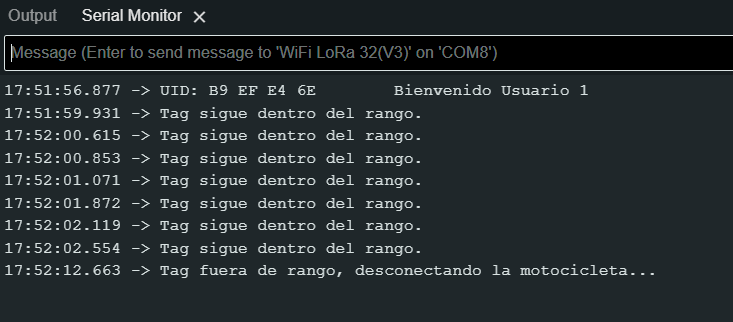
\includegraphics[width=\textwidth]{./capitulo_05/imagen/rfidprueba.png}
\caption{Prueba del módulo RFID.\label{fig:rfid}}
\end{center}
\end{minipage}
\end{figure}

En la Tabla \ref{tab:pruebas_uid}, se puede observar el número de pruebas realizadas para cada versión del código, así como los resultados obtenidos en términos de detección y comparación del UID de las tarjetas y llaveros RFID. Esta información proporciona una visión general del desempeño y funcionamiento del sistema en cada fase del desarrollo.

\begin{table}[H]
\centering
\renewcommand{\arraystretch}{1.3} % Ajusta el espacio entre filas
\caption{Resultados de las pruebas de detección y comparación del UID}
\label{tab:pruebas_uid}
%\begin{tabularx}{\textwidth}{|X|c|c|c|}
\begin{tabular}{|p{3cm}|p{2.65cm}|p{2cm}|p{2.4cm}|}
\hline
\textbf{Versión del Código} & \textbf{Total de Pruebas} & \textbf{Pruebas Exitosas} & \textbf{Pruebas Fallidas} \\ \hline
Primera versión             & 10                       & 7                         & 3                         \\ \hline
Segunda versión             & 30                       & 25                        & 5                         \\ \hline
%\end{tabularx}
\end{tabular}
\end{table}


Las fallas observadas durante las pruebas fueron esporádicas y se debieron a errores humanos, problemas de conexión y ajustes manuales. En algunos casos, los cables se desconectaron accidentalmente durante el proceso, interrumpiendo temporalmente la comunicación del sistema. Otras fallas, aunque puntuales, estuvieron relacionadas con errores en el código que afectaron la detección y comparación del UID. Además, se identificaron dificultades al mantener el tag en posición fija con la mano, lo que ocasionó lecturas inestables en ciertos momentos.


\subsection{Pruebas del Módulo de captura y transmisión de datos}

Se llevaron a cabo pruebas específicas por separado para evaluar la capacidad del sistema en la captura de las coordenadas del módulo GNSS  y su transmisión a través de la red LoRaWAN utilizando la consola Helium. En esta fase, se validó la correcta conexión a un hotspot, así como la correcta recepción de las coordenadas y la recepción de paquetes de datos en condiciones de laboratorio. Las pruebas se dividieron en tres partes, descritas a continuación:

\begin{itemize}
\item  Prueba del módulo GNSS.
\item  Prueba del módulo LoRa del Heltec.
\item  Prueba de captura y transmisión de datos de localización.
\end{itemize}

\subsubsection{Prueba del módulo GNSS} 
En la primera implementación del código, se utilizó únicamente el módulo GNSS conectado a la placa de desarrollo Heltec WiFi LoRa 32 V3. El objetivo fue obtener datos de ubicación y verificar que el sistema pudiera capturar correctamente las coordenadas en tiempo real. Durante esta prueba, se evaluó la precisión de las coordenadas obtenidas, asegurando que fueran consistentes y confiables.
En la figura \ref{fig:gnss}, se puede observar como se obtuvo las coordenadas por monitor serial de la ubicación estática.

\begin{figure}[H]
\leavevmode
\begin{minipage}{\textwidth}
\begin{center}
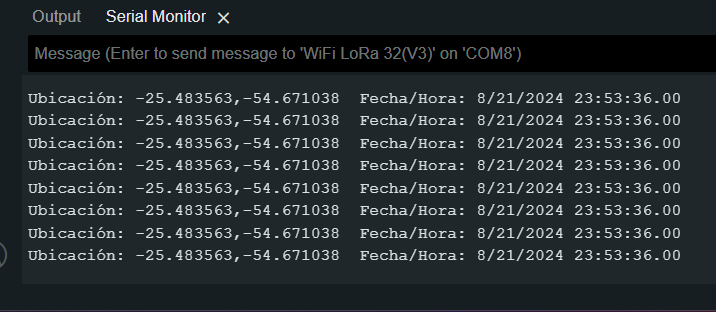
\includegraphics[width=\textwidth]{./capitulo_05/imagen/gnss.png}
\caption{Pruebas del módulo GNSS.\label{fig:gnss}}
\end{center}
\end{minipage}
\end{figure}


Luego, se tomaron las coordenadas obtenidas del módulo GNSS y se verificó su precisión utilizando Google Maps \cite{Google_Maps}. Este paso permitió corroborar la ubicación detectada por el sistema y evaluar la exactitud de la geolocalización en comparación con un dispositivo de referencia. Para ello, se utilizó un teléfono convencional de la marca Xiaomi con modelo Mi 11 Lite, mediante el cual se consultó la ubicación actual del lugar. Este proceso brindó un punto de comparación en cuanto a la precisión del módulo GNSS frente al teléfono, permitiendo analizar posibles diferencias en la exactitud de las coordenadas reportadas por ambos dispositivos.
En las figuras \ref{fig:google} y \ref{fig:telefono}, se muestran, respectivamente, las ubicaciones obtenidas con el módulo GNSS y con el teléfono, facilitando así la visualización comparativa de la precisión entre ambas lecturas.


\begin{figure}[H]
\leavevmode
\begin{minipage}{\textwidth}
\begin{center}
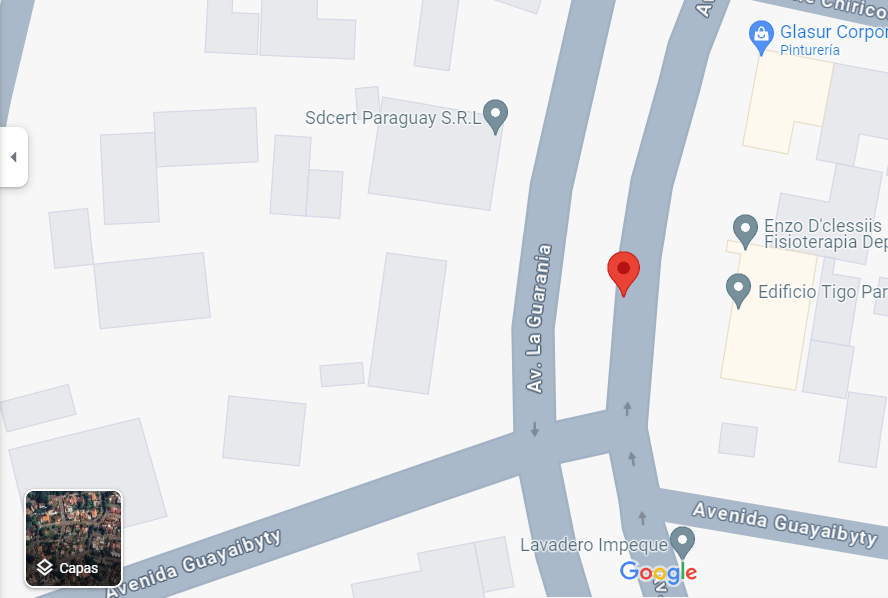
\includegraphics[width=0.8\textwidth]{./capitulo_05/imagen/googlemaps.png}
\caption{Comprobación de las coordenadas del módulo GNSS.\label{fig:google}}
\end{center}
\end{minipage}
\end{figure}


\begin{figure}[H]
\leavevmode
\begin{minipage}{\textwidth}
\begin{center}
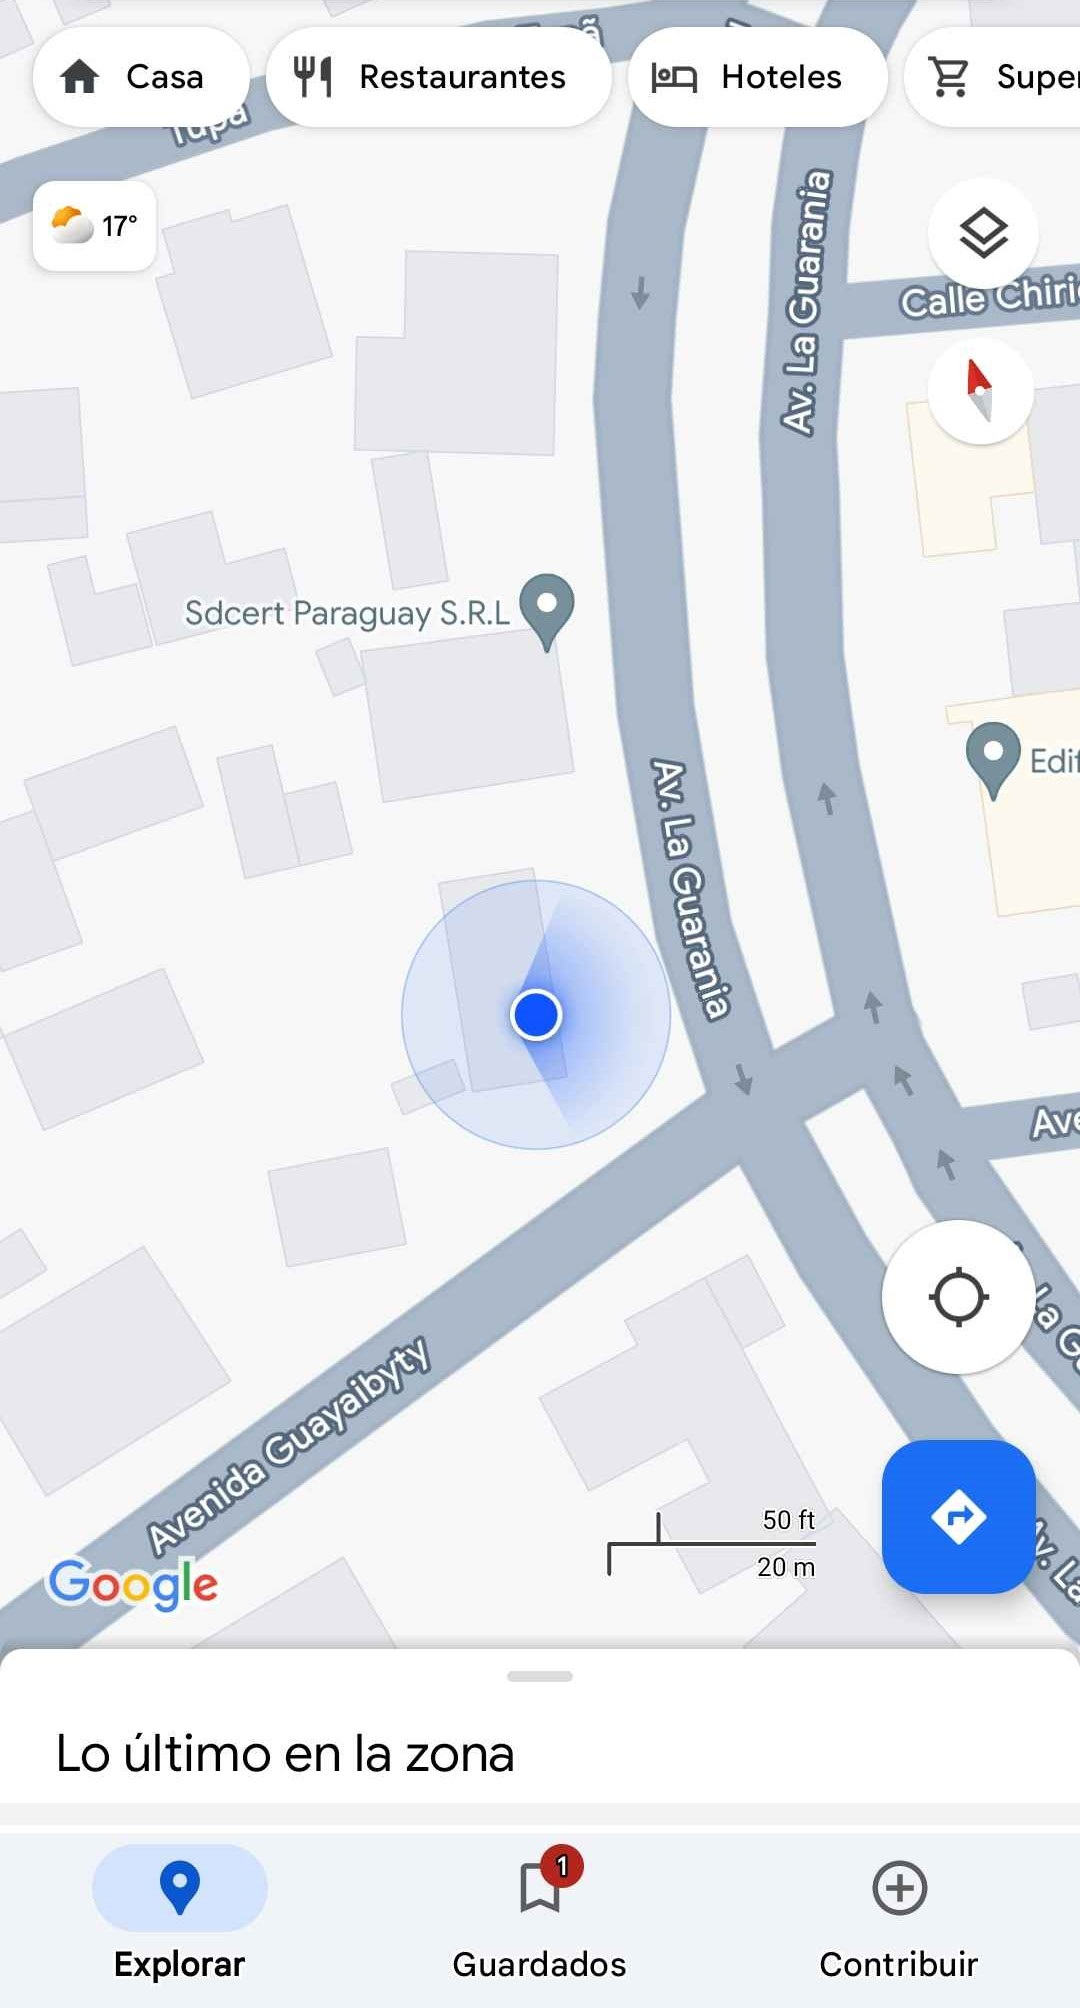
\includegraphics[width=0.4\textwidth]{./capitulo_05/imagen/telefono.jpg}
\caption{Comprobación con teléfono convencional.\label{fig:telefono}}
\end{center}
\end{minipage}
\end{figure}

A partir de la comparación de las ubicaciones obtenidas, se pudo observar una diferencia de aproximadamente 33 metros entre las coordenadas reportadas por el módulo GNSS y el teléfono Xiaomi Mi 11 Lite. Esta variación es una medida importante que permite evaluar la precisión del módulo GNSS en relación con un dispositivo de uso cotidiano, como el teléfono, que emplea servicios de localización basados en múltiples satélites y redes de datos.\\


Es importante destacar que estas pruebas iniciales se realizaron dentro de un recinto cerrado, lo cual pudo haber limitado la precisión del módulo GNSS debido a interferencias o bloqueos de señal. Posteriormente, se realizaron pruebas en un espacio abierto, donde la precisión del módulo mejoró notablemente. La exactitud rondó entre los 4 y 6 metros en promedio, con un error máximo de 8 metros, como se observa en la Figura \ref{fig:google-earth}, que muestra la distancia medida en Google Earth \cite{googleearth2024}, para dos puntos obtenidos.

\begin{figure}[H]
    \centering
    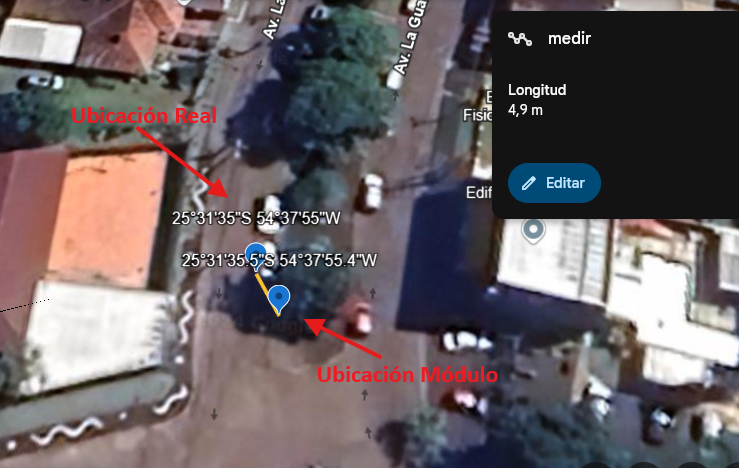
\includegraphics[width=0.8\textwidth]{./capitulo_05/imagen/googleearth.png}
    \caption{Medición de distancias con Google Earth - Coordenadas específicas.}
    \label{fig:google-earth}
\end{figure}



Para validar estas distancias, se utilizó la herramienta Omni Calculator \cite{omnicalculator2024}, con la cual se calculó la separación exacta entre las coordenadas obtenidas. El resultado de esta validación se detalla en la Figura \ref{fig:omni-calculator}, que confirma una diferencia de 4.9 metros entre las posiciones reportadas.


\begin{figure}[H]
    \centering
    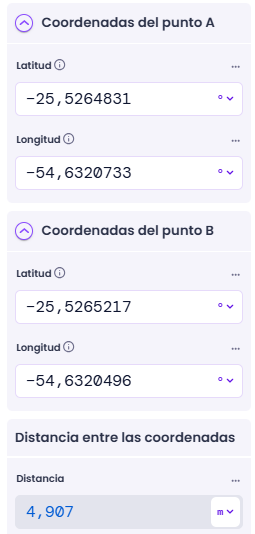
\includegraphics[width=0.3\textwidth]{./capitulo_05/imagen/calculad.png}
    \caption{Distancia calculada con Omni Calculator.}
    \label{fig:omni-calculator}
\end{figure}

En la Figura \ref{fig:multiple-puntos} se ilustran varias ubicaciones adquiridas durante las pruebas en un espacio abierto, demostrando la consistencia de las coordenadas registradas por el módulo GNSS. Estas mediciones fueron esenciales para comprobar la precisión del módulo .



\begin{figure}[H]
    \centering
    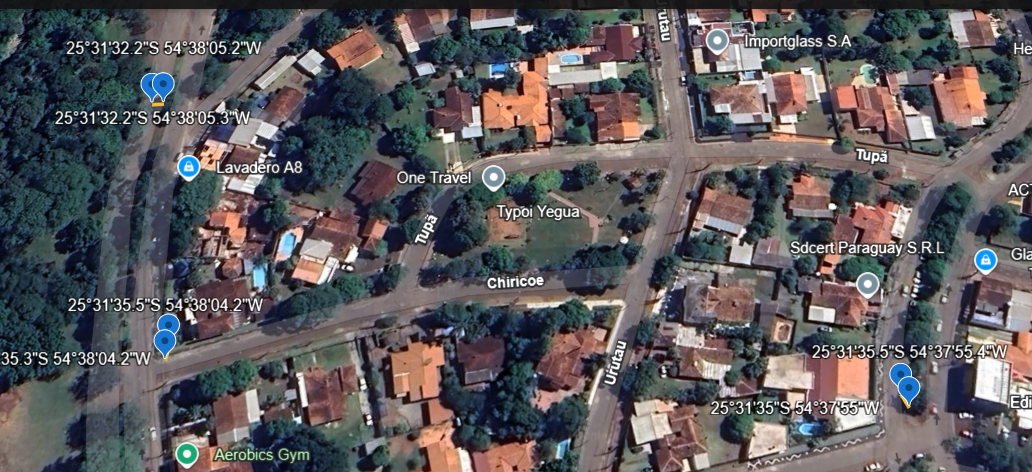
\includegraphics[width=0.9\textwidth]{./capitulo_05/imagen/variascoord.png}
    \caption{Pruebas de ubicación en Google Earth con múltiples puntos adquiridos.}
    \label{fig:multiple-puntos}
\end{figure}

\subsubsection{Prueba del módulo LoRa} 
En la figura \ref{fig:uplink}, se puede observar como se establecio la conexión exitosamente, se pudo observar en la consola como se realizaban las peticiones y los envios uplink. La consola mostró en tiempo real los datos transmitidos desde el dispositivo, confirmando que los mensajes uplink eran recibidos y procesados correctamente por el servidor.
En la segunda implementación, se centró exclusivamente en la funcionalidad de LoRaWAN. Se verificó si el sistema podía enviar correctamente solicitudes de conexión a la red y transmitir mensajes. Esta prueba fue crucial para asegurarse de que el módulo LoRa estuviera configurado correctamente y pudiera establecer comunicación con la red Helium \cite{Helium_Console}, garantizando así que el sistema estuviera listo para la transmisión de datos.

\begin{figure}[H]
\leavevmode
\begin{minipage}{\textwidth}
\begin{center}
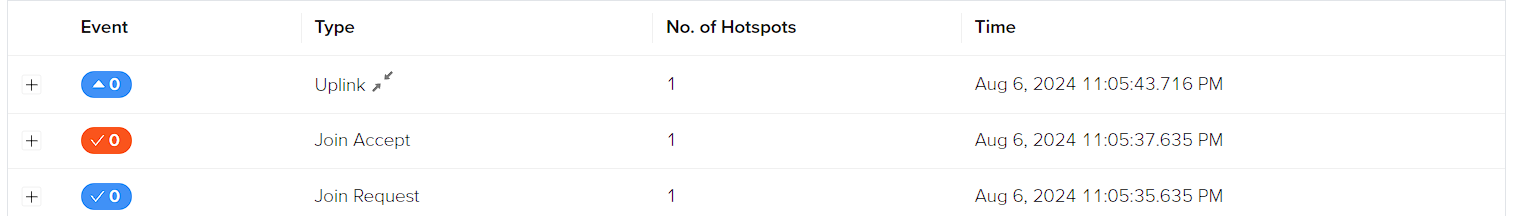
\includegraphics[width=\textwidth]{./capitulo_05/imagen/uplink.png}
\caption{Visualización en la consola helium, mensaje de conexión y subida.\label{fig:uplink}}
\end{center}
\end{minipage}
\end{figure}

La consola también permitió visualizar a qué hostpot se conectó el dispositivo y con cuál realizó el envío de mensajes. Como se muestra en la figura \ref{fig:hostpot}.

\begin{figure}[H]
\leavevmode
\begin{minipage}{\textwidth}
\begin{center}
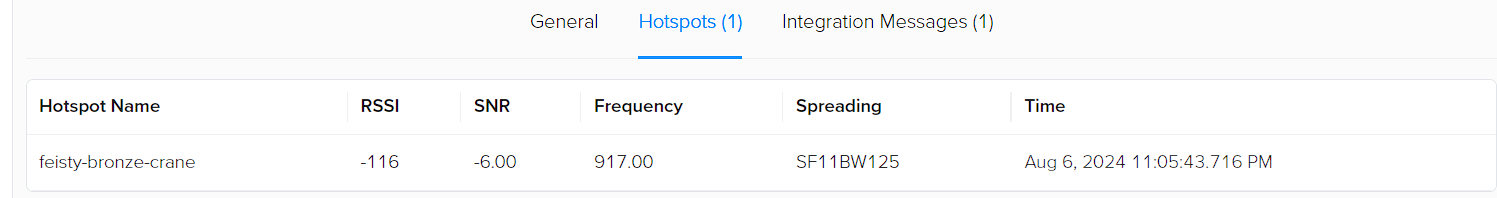
\includegraphics[width=\textwidth]{./capitulo_05/imagen/hostpot.png}
\caption{Visualización en la consola helium.\label{fig:hostpot}}
\end{center}
\end{minipage}
\end{figure}

Con esta información, se utilizó el mapa de Helium \cite{Helium_Explorer}, para identificar la ubicación exacta del hotspot, lo que permitió estimar la distancia desde la cual el dispositivo podía conectarse. Esto facilitó la evaluación de la cobertura y el alcance de la red en el área de prueba, como se puede observa en las siguientes figuras \ref{fig:coverage} y \ref{fig:maps}.

\begin{figure}[H]
\leavevmode
\begin{minipage}{\textwidth}
\begin{center}
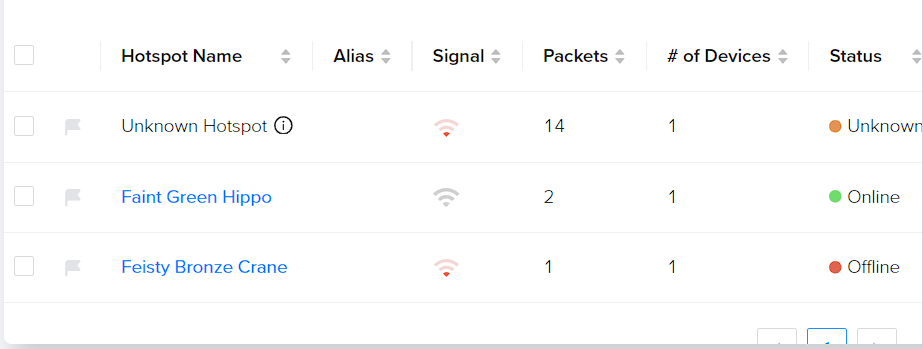
\includegraphics[width=\textwidth]{./capitulo_05/imagen/Coverage.png}
\caption{Visualización de cobertura en la consola helium.\label{fig:coverage}}
\end{center}
\end{minipage}
\end{figure}

\begin{figure}[H]
\leavevmode
\begin{minipage}{\textwidth}
\begin{center}
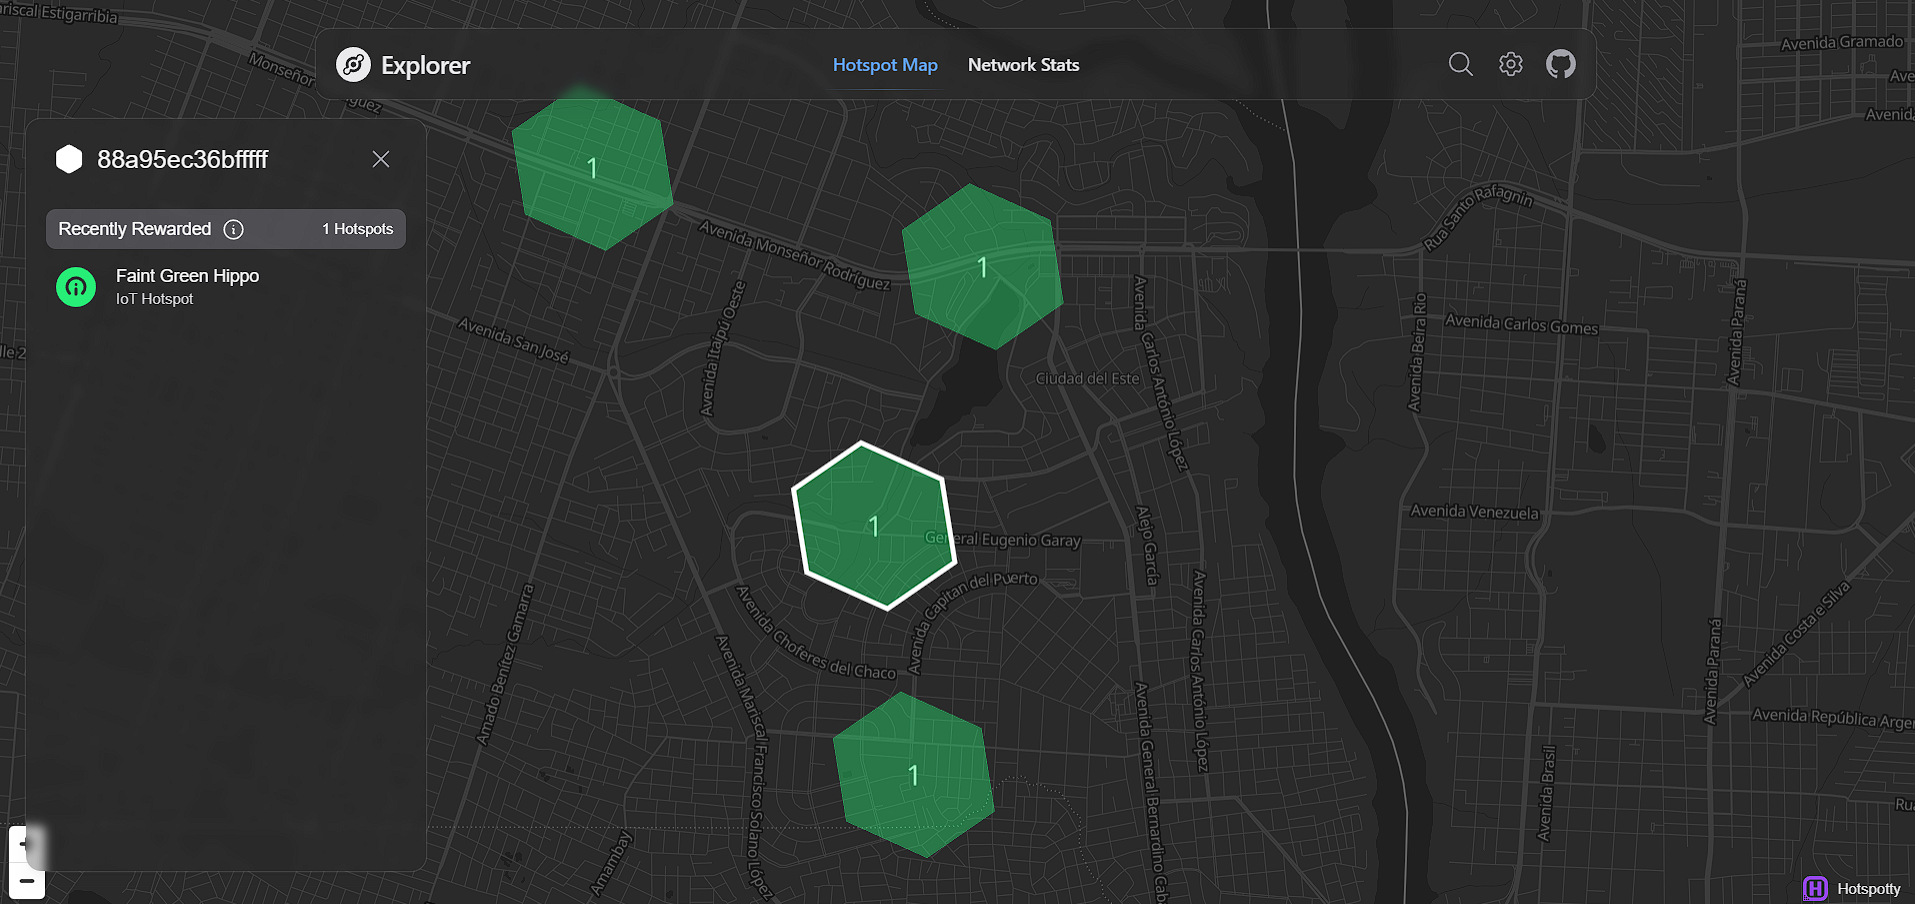
\includegraphics[width=\textwidth]{./capitulo_04/imagen/maps.png}
\end{center}
\caption{Visualización en la página helium maps.\label{fig:maps}}
\end{minipage}
\end{figure}

Esta información adicional facilitó la verificación del funcionamiento de la red y permitió asegurar que la comunicación entre el dispositivo y el hotspot se estaba realizando de manera efectiva.

\subsubsection{Prueba de captura y transmisión de datos de localización} 
En la tercera implementación, se combinó la obtención de datos de localización del módulo GNSS con el envío de estos datos a través de LoRaWAN. Durante esta prueba, se verificó la correcta transmisión de los payloads que contenían las coordenadas GNSS, asegurando que no hubiera pérdida de datos en el proceso. Además, se realizó una decodificación manual del payload para validar su contenido. Se analizó la recepción de los datos en el servidor, confirmando que las coordenadas se enviaran y registraran sin errores. En la Figura \ref{fig:Json}, se muestra la estructura del archivo JSON que se descargó de la consola Helium, donde se registran todas las acciones realizadas.

\begin{figure}[H]
\leavevmode
\begin{minipage}{\textwidth}
\begin{center}
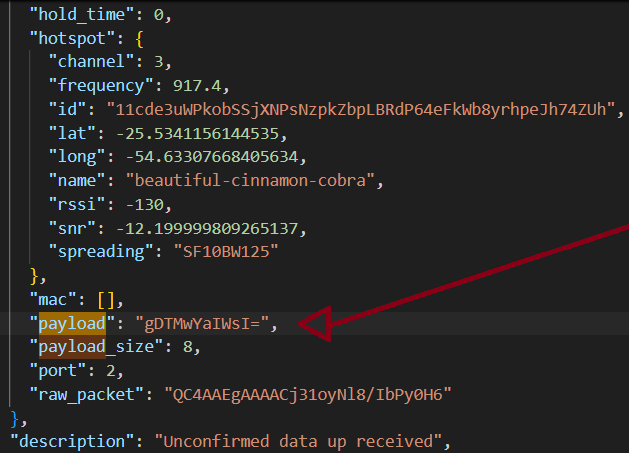
\includegraphics[width=\textwidth]{./capitulo_05/imagen/payload.png}
\caption{Estructura del Mensaje enviado, donde 
payload serían las coordenadas en Base64.\label{fig:Json}}
\end{center}
\end{minipage}
\end{figure}

Para validar la precisión de las coordenadas GNSS transmitidas, se siguieron los siguientes pasos para decodificar el mensaje recibido:


Por ejemplo, el mensaje gDTMwYaIWsI= se decodifica a: Latitud: -25.5256, Longitud: -54.6333.
Para la decodificación Base 64, se utilizó una herramienta en línea, como Base64 Decode \cite{Cryptii_Base64_to_Hex}, para decodificar el mensaje. Este proceso convierte el mensaje codificado en una serie de bytes en formato hexadecimal, lo que facilita su interpretación. Luego se dividieron los primeros 4 bytes del mensaje para obtener la latitud y los siguientes 4 bytes para la longitud. Para convertir estos bytes en números flotantes (float), se utilizó una calculadora en línea, como Hex Convert \cite{SCADACore_Hex_Converter}. Esta herramienta permite convertir el formato hexadecimal en un valor numérico que puede ser interpretado como coordenadas.


En las Figuras \ref{fig:base64a} y \ref{fig:base64b}, se muestra el proceso de conversión utilizando la herramienta mencionada, ilustrando cómo se obtuvieron las coordenadas a partir del mensaje recibido.

\begin{figure}[H]
\leavevmode
\begin{minipage}{\textwidth}
\begin{center}
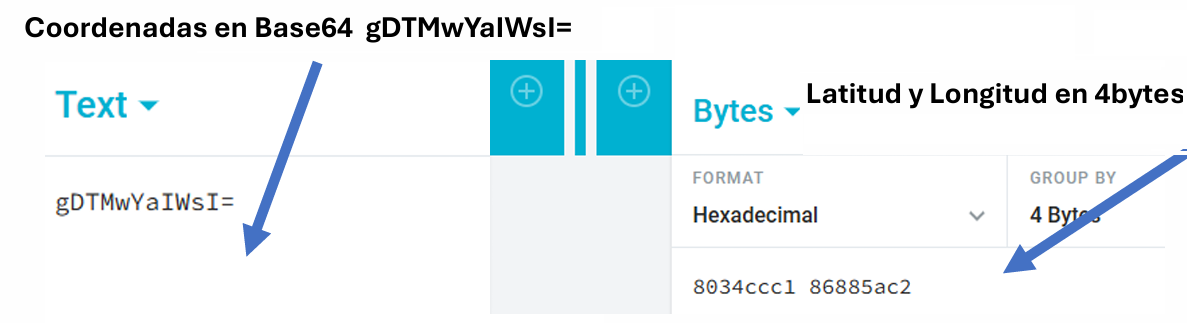
\includegraphics[width=\textwidth]{./capitulo_05/imagen/base64a.png}
\caption{Interpretación de Base64 a Hexadecimal.\label{fig:base64a}}
\end{center}
\end{minipage}
\end{figure}

\begin{figure}[H]
\leavevmode
\begin{minipage}{\textwidth}
\begin{center}
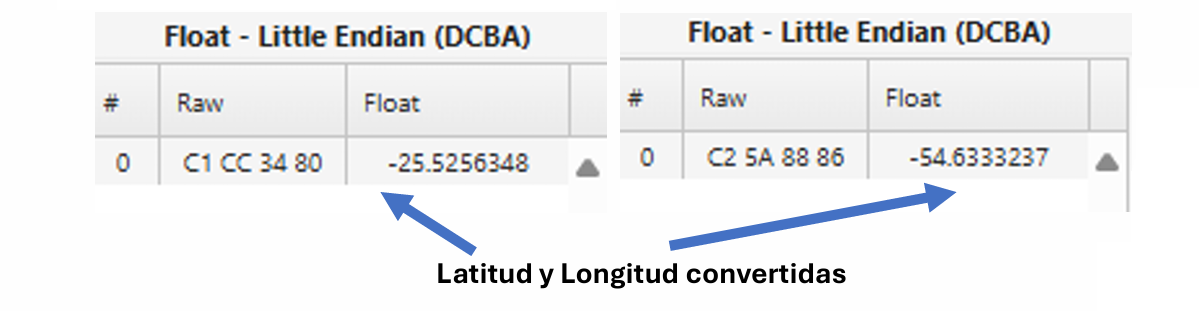
\includegraphics[width=\textwidth]{./capitulo_05/imagen/base64b.png}
\caption{Interpretación de las coordenadas de latitud y longitud transmitidas.\label{fig:base64b}}
\end{center}
\end{minipage}
\end{figure}

\subsection{Pruebas del Módulo de Interfaz Gráfica y Monitoreo}
El módulo de Interfaz Gráfica y Monitoreo se configuró para recibir y procesar datos en tiempo real de la ubicación y estado de un dispositivo prototipo. Durante las pruebas, se verificaron las siguientes funcionalidades clave: transmisión de datos, visualización en mapas interactivos, almacenamiento de datos en series temporales, y decodificación de mensajes en formato \textit{Base64}.

\subsubsection{Transmisión y visualización de datos}

El dispositivo prototipo fue configurado en la consola de \textit{ThingsBoard} para enviar datos de telemetría, tales como latitud, longitud, y eventos de usuario. Los datos se transmitieron a través del protocolo \textit{MQTT} y fueron correctamente registrados en el tablero de control del sistema, donde se visualizan en tiempo real en un mapa \textit{OpenStreet} (ver Figura~\ref{fig:mapopen}).
\begin{figure}[H]
\leavevmode
%\begin{minipage}{\textwidth}
\begin{center}
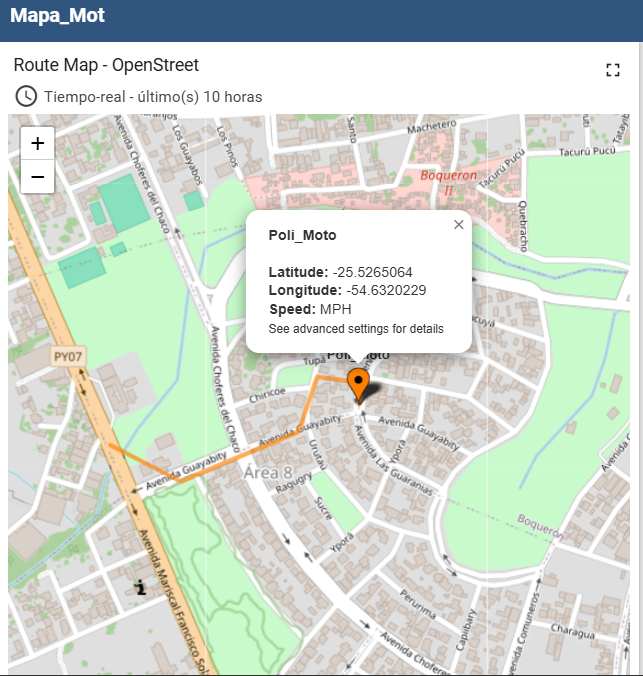
\includegraphics[width=0.7\textwidth]{./capitulo_05/imagen/resmon/mapa2.png}
\caption{Visualización de la ubicación en el mapa \textit{OpenStreet} con trayectoria.\label{fig:mapopen}}
\end{center}
%\end{minipage}
\end{figure}
\subsubsection{Almacenamiento en tablas de series temporales}

La telemetría se almacenó en una tabla de series de tiempo que registró cada evento, permitiendo un análisis detallado de la trayectoria y actividad del dispositivo (ver Figura~\ref{fig:tempser}). Esto proporcionó un historial de datos que facilita la trazabilidad y auditoría de la ubicación del dispositivo en distintos momentos del día.

\begin{figure}[H]
\leavevmode
\begin{minipage}{\textwidth}
\begin{center}
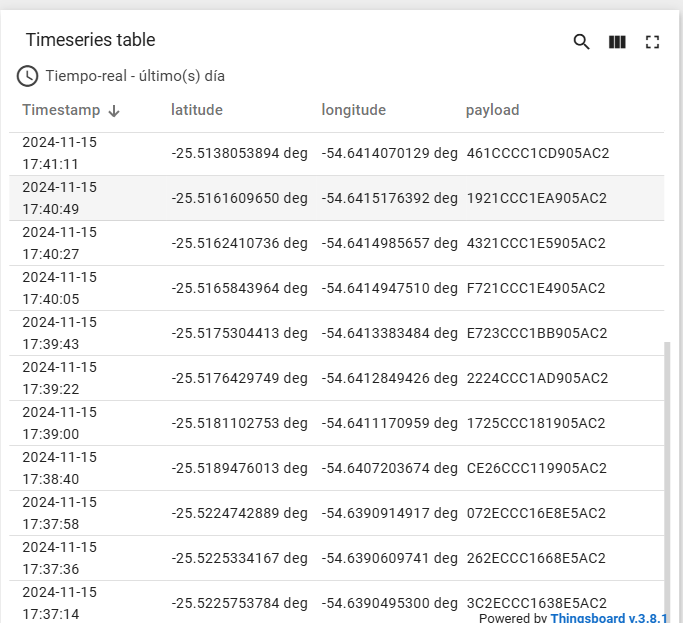
\includegraphics[width=0.75\textwidth]{./capitulo_05/imagen/resmon/timeserie.png}
\caption{Series temporales de telemetría.\label{fig:tempser}}
\end{center}
\end{minipage}
\end{figure}
\subsubsection{Pruebas de decodificación y transformación de datos}

Para evaluar la correcta interpretación de mensajes enviados al sistema, se llevaron a cabo una serie de pruebas utilizando dos scripts desarrollados en \textit{JavaScript}. Estas pruebas se diseñaron para asegurar la decodificación precisa de los datos transmitidos en formato \textit{Base64} y su posterior interpretación en valores útiles para el sistema.

El proceso se dividió en dos etapas principales de prueba. En la primera etapa, se probó un script encargado de transformar los datos enviados en formato \textit{Base64} a valores hexadecimales (ver Figura~\ref{fig:to64}). Este script se verificó con mensajes simulados de distintos tamaños y contenido. Se realizaron 5 pruebas, cada una con un mensaje diferente, asegurando que los valores obtenidos fueran consistentes con los datos esperados.

En la segunda etapa, se utilizó un script adicional que interpretaba los valores hexadecimales obtenidos en la etapa previa. Este script clasificaba los datos según el tamaño del mensaje decodificado:

\begin{itemize}
    \item Mensajes de 2 \textit{bytes} representaban eventos, como alertas de desconexión o intentos de acceso no autorizado.
    \item Mensajes de 4 \textit{bytes} representaban eventos, como de acceso de usuarios autorizados.    
    \item Mensajes de 8 \textit{bytes} correspondían a telemetrías de ubicación, como coordenadas de latitud y longitud.

\end{itemize}

Durante esta etapa, se realizaron 10 pruebas para verificar la capacidad del sistema de manejar una variedad de tamaños y contenidos diferentes en los mensajes. Los resultados de todas las pruebas fueron exitosos, demostrando es capaz de interpretar y clasificar correctamente los datos enviados. Un ejemplo de este proceso puede observarse en la Figura~\ref{fig:tohex}, donde se muestra la interpretación de un mensaje hexadecimal como denegación de acceso no autorizado.



\begin{figure}[H]
\leavevmode
\begin{minipage}{\textwidth}
\begin{center}
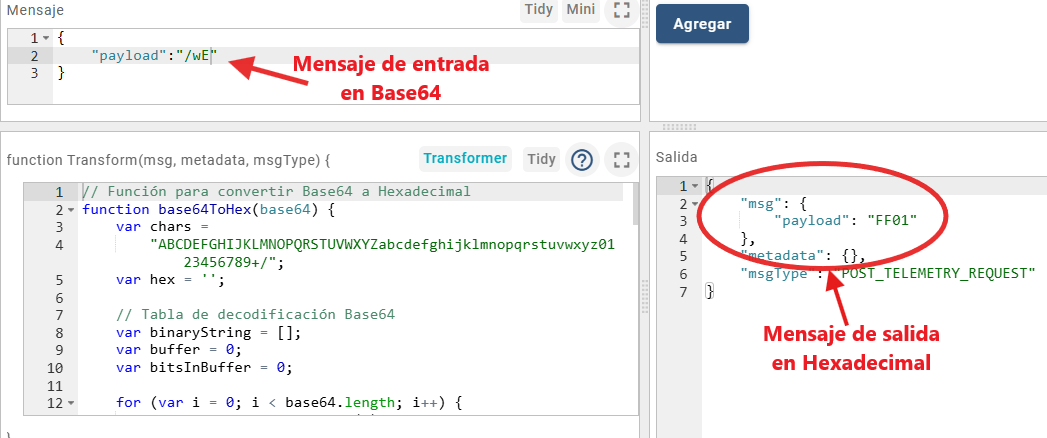
\includegraphics[scale=0.5]{./capitulo_05/imagen/resmon/64to (1).png}
\caption{Prueba de decodificación de mensajes en formato \textit{Base64} a valores hexadecimales.\label{fig:to64}}
\end{center}
\end{minipage}
\end{figure}



\begin{figure}[H]
\leavevmode
\begin{minipage}{\textwidth}
\begin{center}
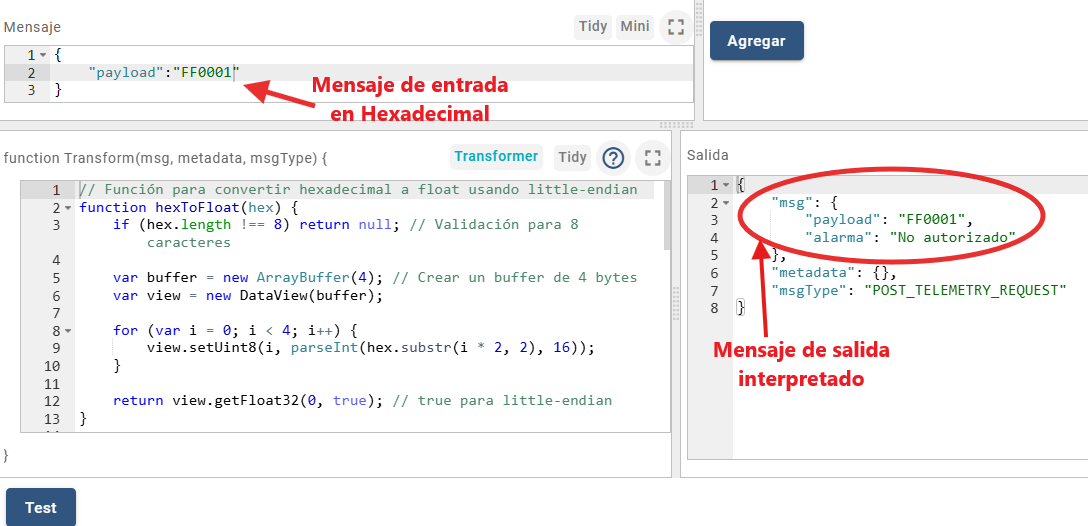
\includegraphics[scale=0.5]{./capitulo_05/imagen/resmon/hextto (1).png}
\caption{Prueba de interpretación de valores hexadecimales según su tamaño.\label{fig:tohex}}
\end{center}
\end{minipage}
\end{figure}

Para garantizar la precisión de las pruebas, se utilizó \textit{Mosquitto} como herramienta para enviar mensajes simulados al sistema (ver Figura~\ref{fig:mosqu_p}). Esta herramienta permitió verificar el flujo completo de transmisión.

Todos los resultados confirmaron el correcto funcionamiento del sistema, logrando interpretar los datos en tiempo real de manera eficiente y confiable.


\begin{figure}[H]
\leavevmode
\begin{minipage}{\textwidth}
\begin{center}
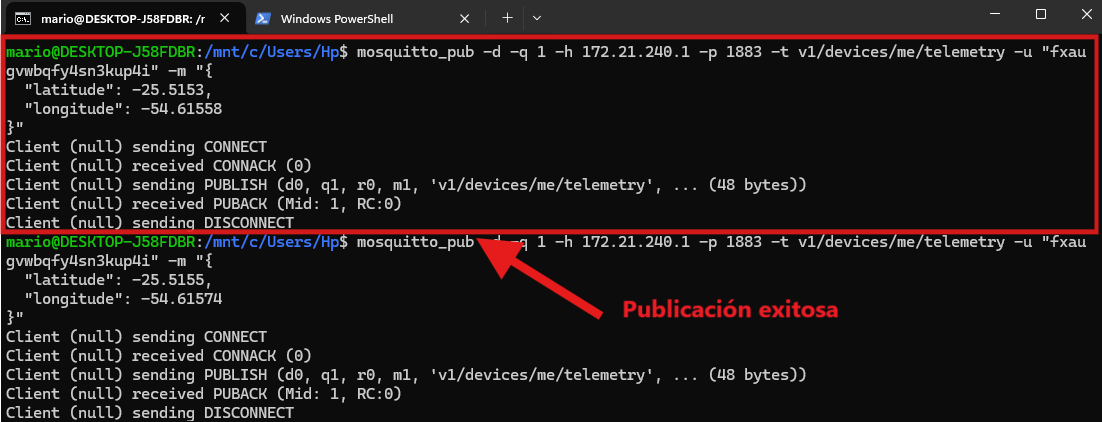
\includegraphics[width=\textwidth]{./capitulo_05/imagen/resmon/mosquitt.png}
\caption{Uso de \textit{Mosquitto} para simular mensajes durante las pruebas.\label{fig:mosqu_p}}
\end{center}
\end{minipage}
\end{figure}

\subsubsection{Resultados de la integración entre ThingsBoard y Helium }

En la Figura~\ref{fig:hel_tb} se observa el resultado del proceso de integración entre ThingsBoard y la red Helium mediante el protocolo \textit{MQTT}. Este proceso consistió en la recepción y procesamiento de cada mensaje enviado desde lel dispositivo conectado. 

\begin{figure}[H]
\leavevmode
\begin{minipage}{\textwidth}
\begin{center}
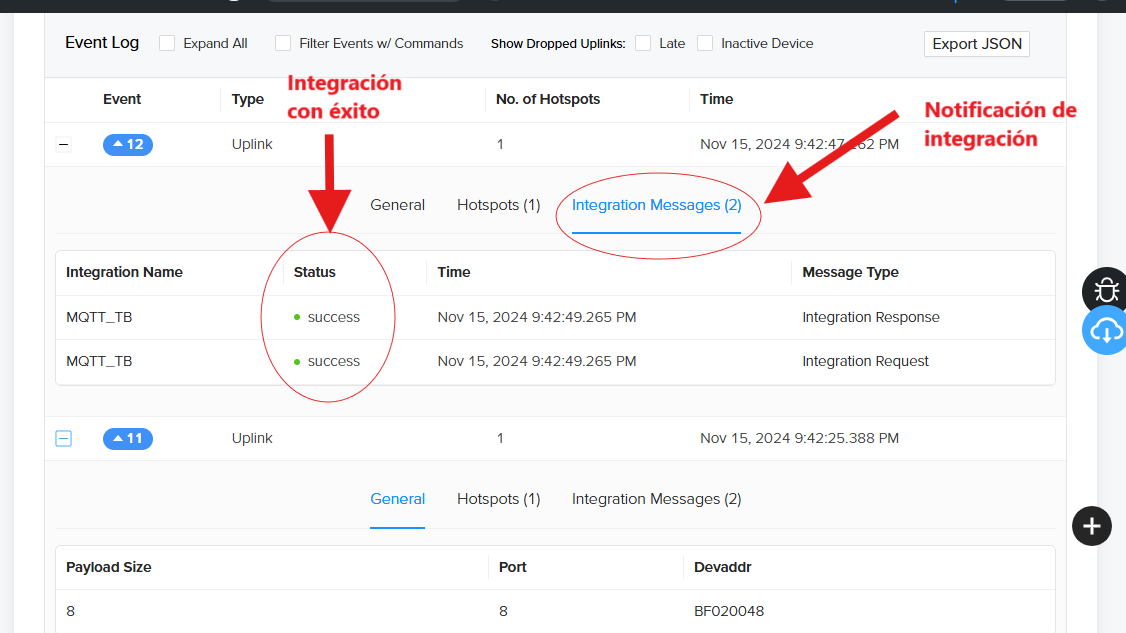
\includegraphics[width=0.9\textwidth]{./capitulo_05/imagen/resmon/integra2c.png}
\caption{Integración Helium-ThingsBoards.\label{fig:hel_tb}}
\end{center}
\end{minipage}
\end{figure}

De los más de 120 mensajes transmitidos, un total de 8 mensajes fallaron al momento de integrarse, lo que representa un porcentaje de efectividad del 93.33\% en la integración.

A pesar de estas fallas, los mensajes que sí lograron ser transmitidos exitosamente fueron interpretados y decodificados con un 100\% de efectividad. Esto incluye tanto la transformación de los datos de formato \textit{Base64} a hexadecimales como su interpretación en valores útiles para el sistema, validando el correcto funcionamineto del módulo.




\subsection{Integración del sistema completo}
En esta fase, se realizaron pruebas específicas para validar la integración y el correcto funcionamiento de todos los módulos necesarios para el sistema: RFID, GNSS y LoRaWAN, utilizando las placas de desarrollo ESP-WROOM-32 y Heltec WiFi LoRa 32 V3. El objetivo principal fue asegurar la operación conjunta de estos módulos en el sistema, comprobando la funcionalidad de identificación mediante RFID, la transmisión de datos de ubicación y el envío de información por la red LoRaWAN. Las pruebas se desarrollaron en tres etapas, detalladas a continuación:

\subsubsection {Primera Prueba: Comunicación entre las placas de desarrollo (ESP-WROOM-32 y Heltec WiFi LoRa 32 V3)}
Esta prueba inicial consistió en establecer la comunicación entre ambas placas mediante el protocolo UART, con el módulo RFID conectado al ESP-WROOM-32. El sistema transmitió datos de identificación desde el módulo RFID al Heltec WiFi LoRa 32 V3, validando la presencia del UID autorizado. Además, se comprobó que esta transmisión no interrumpiera la conexión con la red LoRaWAN, manteniendo la integridad de los datos y la estabilidad de la comunicación entre los dispositivos.

\subsubsection {Segunda Prueba: Integración del Módulo GNSS}
En esta etapa, se implementó la versión 2 del código, que integraba el módulo GNSS junto con el módulo RFID. La prueba se orientó a evaluar la transmisión de los datos recolectados, donde:

El UID autorizado fue enviado en formato hexadecimal.
Otros datos de ejemplo fueron incluidos en la transmisión para verificar la estructura de los mensajes.
Las coordenadas GPS fueron convertidas a un formato adecuado, preparadas como un arreglo de bytes para ser enviadas por LoRaWAN.
\subsubsection {Tercera Prueba: Evaluación de las Funciones de Envío de Datos Completos}
En la última fase, se probó la versión 3 del código, que incluyó el flujo completo de detección RFID, obtención de coordenadas GNSS y envío de datos a través de LoRaWAN. En esta prueba se evaluaron las siguientes condiciones:
\begin{itemize}
\item Detección RFID: El sistema identificó la presencia de un tag RFID autorizado, enviando el UID a través de LoRaWAN en el caso de una identificación válida.
\item Envío de Datos por LoRaWAN: Dependiendo del tipo de mensaje seleccionado, el sistema envió el UID del RFID, otros datos de prueba o, en caso de estar disponibles, las coordenadas.
\item Ciclo de LoRaWAN: El dispositivo siguió un ciclo de transmisión periódica, entrando en modo de suspensión tras cada envío, optimizando así el consumo energético.
\item Validación de Coordenadas: Se verificó que el dispositivo obtuviera coordenadas válidas y las transmitiera en el siguiente ciclo de envío, asegurando que no hubiera pérdida de datos en la transmisión.
\end{itemize}

Los resultados de las pruebas realizadas para las tres versiones del código se resumen en la Tabla \ref{tab:pruebacompleta}.

\begin{table}[H]
\centering
\renewcommand{\arraystretch}{1.3} % Ajusta el espacio entre filas
\caption{Resultados de las Pruebas por Versión del Código}
\label{tab:pruebacompleta}
%\begin{tabularx}{\textwidth}{|X|c|c|c|}
\begin{tabular}{|p{3cm}|p{2.65cm}|p{2cm}|p{2.2cm}|}
\hline
\textbf{Versión del Código} & \textbf{Total de Pruebas} & \textbf{Pruebas Exitosas} & \textbf{Pruebas Fallidas} \\ \hline
Primera Versión             & 10                       & 8                         & 2                         \\ \hline
Segunda Versión             & 20                       & 15                        & 5                         \\ \hline
Tercera Versión             & 25                       & 24                        & 1                         \\ \hline
%\end{tabularx}
\end{tabular}
\end{table}


A lo largo de las pruebas realizadas, la evolución del sistema mostró mejoras significativas. En la primera versión, se obtuvieron un 80 \% de éxito y un 20\% de fallos en 10 pruebas. La segunda versión alcanzó un 75\% de éxito y un 25\%  de fallos en 20 pruebas. Finalmente, la tercera versión logró una notable eficiencia con un 96\%  de éxito y solo un 4\%  de fallos en 25 pruebas. 

En la Figura \ref{fig:uid}, se presenta la correcta recepción de los datos de UID, transmitidos como payloads de 4 bytes. En la Figura \ref{fig:cord}, se muestra cómo se recibieron los datos de las coordenadas en los intervalos de tiempo definidos.

\begin{figure}[H]
\leavevmode
\begin{minipage}{\textwidth}
\begin{center}
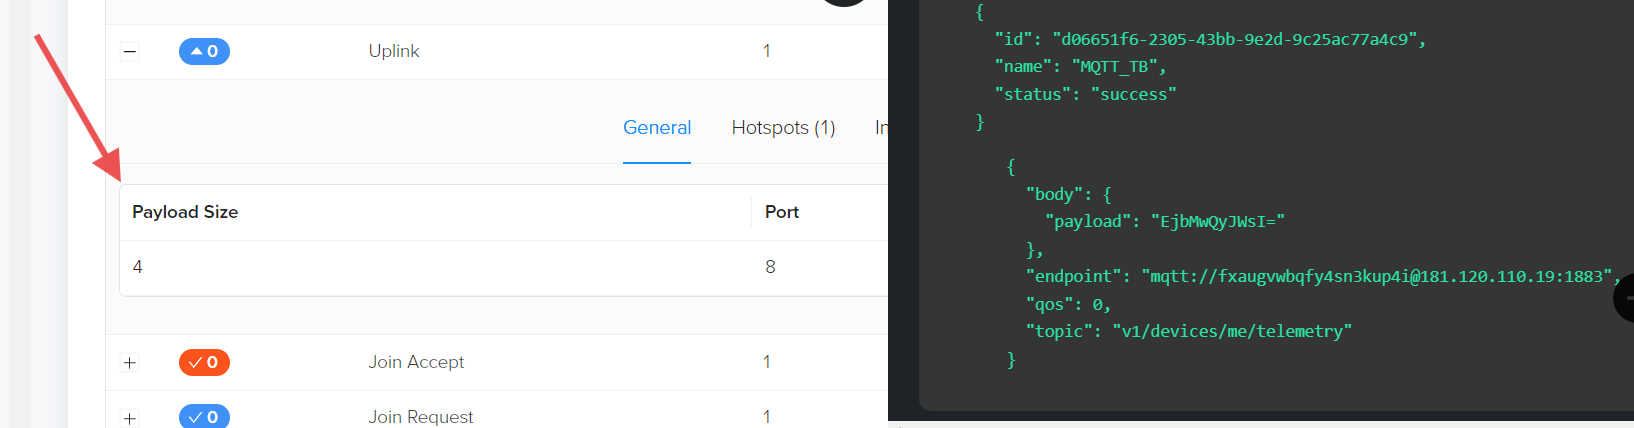
\includegraphics[width=\textwidth]{./capitulo_05/imagen/uid.png}
\caption{Visualización en la consola Helium de los paquetes de datos recibidos del UID.\label{fig:uid}}
\end{center}
\end{minipage}
\end{figure}

\begin{figure}[H]
\leavevmode
\begin{minipage}{\textwidth}
\begin{center}
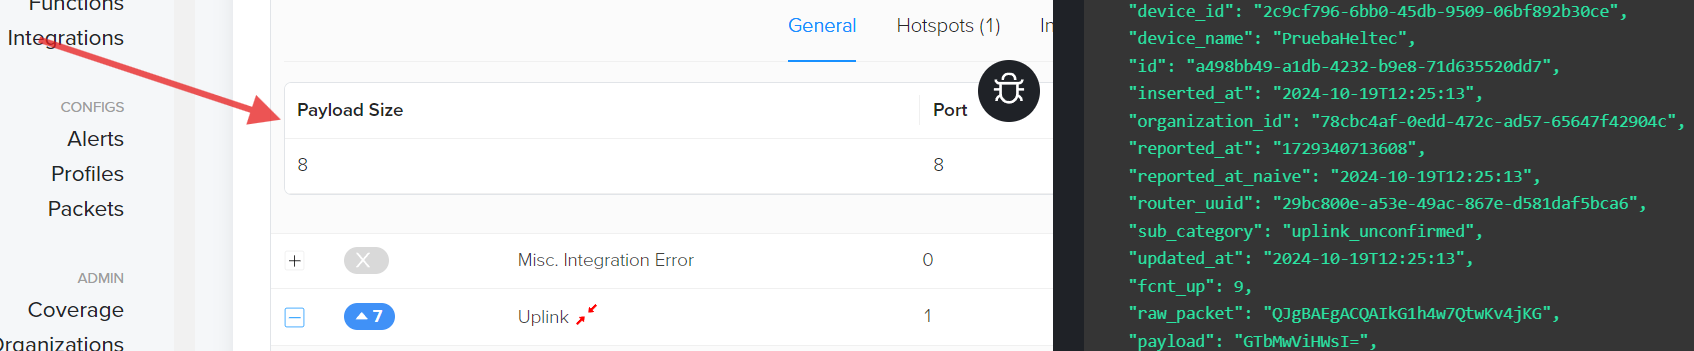
\includegraphics[width=\textwidth]{./capitulo_05/imagen/coord.png}
\caption{Visualización en la  consola Helium de los paquetes de datos recibidos de las coordenadas.\label{fig:cord}}
\end{center}
\end{minipage}
\end{figure}



\section{Pruebas de Campo}

En esta sección, se documentan las pruebas de campo realizadas con una motocicleta Kenton, modelo GL150, equipada con un sistema de encendido \textit{CDI} (Ignición por Descarga de Condensador) y una batería de 12 voltios. Estas pruebas se llevaron a cabo utilizando la última versión del código ajustado, que integra la funcionalidad de corte de energía y arranque controlado mediante el sistema \textit{RFID} y el módulo relé. Además, se evaluó el rendimiento del sistema en movimiento.

\subsection{Evaluación Inicial}

El propósito de las pruebas iniciales fue verificar la integración del sistema y su capacidad para realizar autenticaciones fluidas y sincronizarse adecuadamente con el módulo de corte de energía. Se comprobó que el sistema respondiera de manera precisa a la presencia de un \textit{tag} autorizado, ejecutando el corte de energía al retirarse o ausentarse dicho \textit{tag}. Además, se llevaron a cabo varias pruebas para medir la respuesta del sistema y garantizar su fiabilidad.

En la Figura \ref{fig:esquematico}, se presenta el diagrama esquemático de las conexiones realizadas para la integración del sistema desarrollado en la motocicleta. Este esquema representa la interacción entre los componentes eléctricos de la motocicleta y el prototipo diseñado.

\begin{figure}[H]
\leavevmode
\begin{minipage}{\textwidth}
\begin{center}
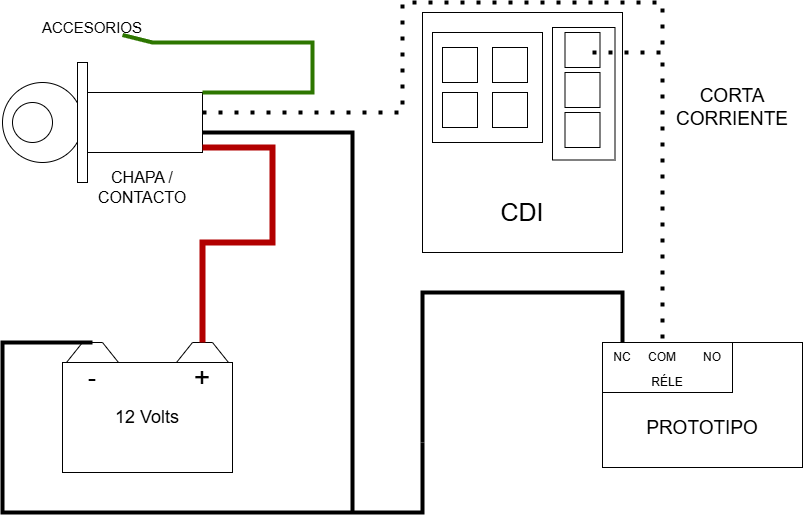
\includegraphics[width=0.7\textwidth]{./capitulo_05/imagen/diagramaesquematico.png}
\caption{Diagrama esquemático de conexiones.\label{fig:esquematico}}
\end{center}
\end{minipage}
\end{figure}

\subsection{Pruebas en Movimiento}

Posteriormente, se realizaron 9 pruebas de campo adicionales para evaluar el comportamiento del sistema en condiciones reales de movimiento. En estas pruebas, se evaluaron las siguientes fases:

\begin{itemize}
    \item \textbf{Conexión a \textit{LoRaWAN} en movimiento:} En tres pruebas específicas, se inició el sistema fuera del área de cobertura de la red \textit{LoRaWAN}, y se comprobó que, al entrar en el rango de la red, el dispositivo lograba realizar el proceso de \textit{join} exitosamente. Todas estas pruebas fueron satisfactorias.
    \item \textbf{Autenticación y arranque del motor:} En cada prueba, se aproximó el \textit{tag RFID} para autenticar al usuario. Aunque en dos pruebas iniciales la lectura del \textit{UID} falló, provocando el apagado inmediato del motor, las pruebas posteriores fueron exitosas, logrando una autenticación fluida y un arranque sin interrupciones.
    \item \textbf{Estabilidad del sistema durante el movimiento:} Durante todas las pruebas, el sistema permaneció operativo, sin desconexiones ni interrupciones, incluso al enfrentarse a cambios de velocidad.
    \item \textbf{Transmisión de datos en tiempo real:} El sistema transmitió correctamente las coordenadas \textit{GPS} y los eventos críticos (autenticación, desconexión, etc.) a la plataforma \textit{ThingsBoard}, donde se visualizaron en tiempo real.
\end{itemize}

En la Figura \ref{fig:trayectoris}, se ilustra una de las trayectorias recogidas durante las pruebas de movimiento, mostrando cómo el sistema registró y transmitió la ubicación de la motocicleta en tiempo real.

\begin{figure}[H]
\leavevmode
\begin{minipage}{\textwidth}
\begin{center}
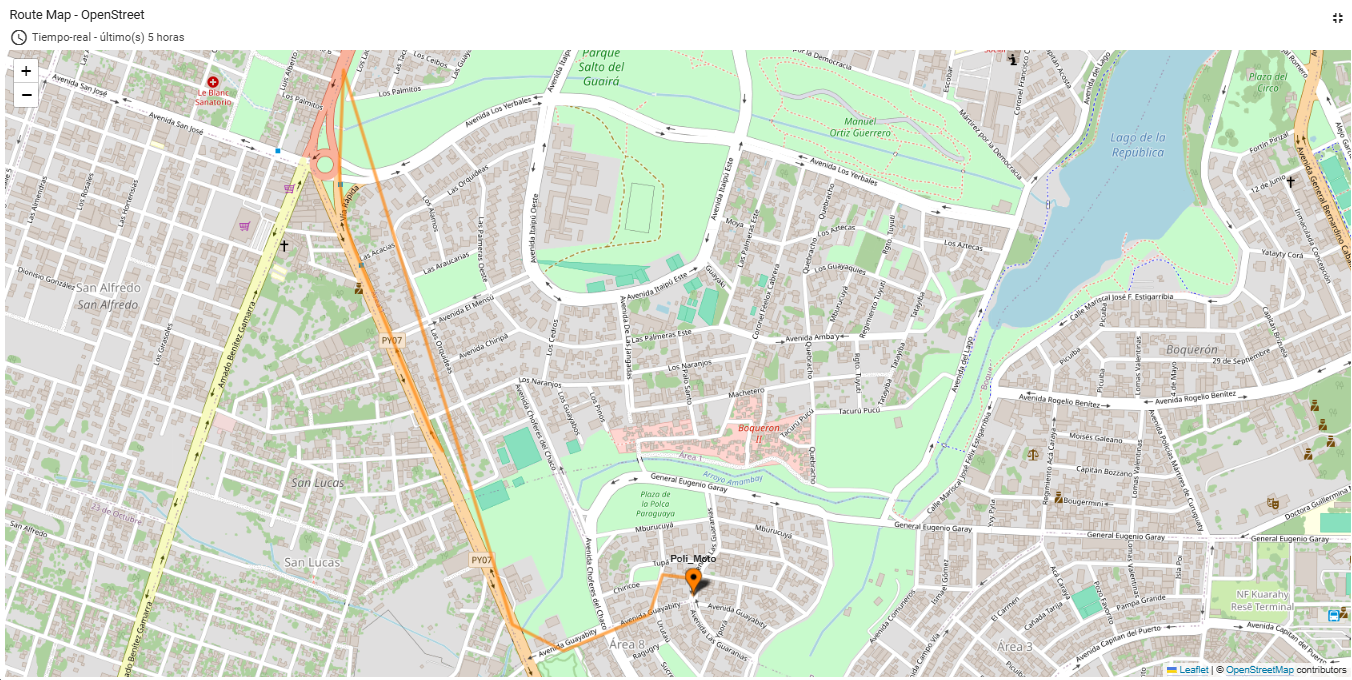
\includegraphics[width=1.0\textwidth]{./capitulo_05/imagen/mapa1.png}
\caption{Trayectoria registrada durante las pruebas de campo.\label{fig:trayectoris}}
\end{center}
\end{minipage}
\end{figure}

\subsection{Resultados Cuantitativos}

En la Tabla \ref{tab:resultable}, se resumen los resultados de las pruebas realizadas, incluyendo autenticaciones exitosas, conexiones a \textit{LoRaWAN} y transmisión de datos durante el movimiento.

\begin{table}[H]
\centering
\renewcommand{\arraystretch}{1.3} % Ajusta el espacio entre filas
\caption{Resultados de las pruebas de campo}
\label{tab:resultable}
\begin{tabular}{|p{1.2cm}|p{2.65cm}|p{2cm}|p{2.4cm}|p{1.6cm}|p{1.7cm}|}
\hline
\textbf{N° de Prueba} & \textbf{Autenticación exitosa} & \textbf{Conexión a LoRaWAN} & \textbf{Transmisión de datos} & \textbf{Sistema estable} & \textbf{Corte al alejar el tag} \\ \hline
1                     & No                             & Sí                          & Sí                            & Sí                      & Sí                              \\ \hline
2                     & No                             & Sí                          & Sí                            & Sí                      & Sí                              \\ \hline
3                     & Sí                             & Sí                          & Sí                            & Sí                      & Sí                              \\ \hline
4                     & Sí                             & Sí                          & Sí                            & Sí                      & Sí                              \\ \hline
5                     & Sí                             & Sí                          & Sí                            & Sí                      & Sí                              \\ \hline
6                     & Sí                             & Sí                          & Sí                            & Sí                      & Sí                              \\ \hline
7                     & Sí                             & Sí                          & Sí                            & Sí                      & Sí                              \\ \hline
8                     & Sí                             & Sí                          & Sí                            & Sí                      & Sí                              \\ \hline
9                     & Sí                             & Sí                          & Sí                            & Sí                      & Sí                              \\ \hline
\end{tabular}
\end{table}


\subsubsection{Porcentajes de Éxito y Fallo}

\begin{itemize}
    \item \textbf{Autenticación exitosa:} De las 9 pruebas realizadas, 7 lograron autenticar correctamente al usuario mediante el \textit{tag RFID}, lo que representa un 77.78\% de éxito. Las dos fallas iniciales, que corresponden al 22.22\% de fallo, se debieron a errores humanos durante el proceso de manejo del sistema, como una posición incorrecta del tag RFID o fallos en su aproximación al lector. Estas situaciones fueron identificadas y corregidas en las pruebas posteriores, logrando resultados exitosos en el resto de las evaluaciones. 
    \item \textbf{Conexión a \textit{LoRaWAN}:} En el 100\% de las pruebas, el dispositivo logró conectarse exitosamente a la red \textit{LoRaWAN}, incluso en condiciones de movimiento y al iniciar fuera del rango de cobertura. Esto demuestra una fiabilidad completa (100\% de éxito) en la capacidad de conexión del sistema.
    \item \textbf{Transmisión de datos:} En todas las pruebas, los datos del sistema, como coordenadas \textit{GPS} y eventos críticos, fueron transmitidos correctamente a la plataforma \textit{ThingsBoard}. Esto refleja un 100\% de éxito en la transmisión de datos.
    \item \textbf{Sistema estable:} Durante todas las pruebas, el sistema permaneció operativo, sin apagarse ni desconectarse de manera inesperada. Esto indica una estabilidad del 100\%.
    \item \textbf{Corte de energía al alejar la tarjeta:} En el 100\% de los casos, el sistema ejecutó correctamente el corte de energía al detectar la ausencia del \textit{tag} autorizado. Este resultado asegura una respuesta fiable del sistema en situaciones de seguridad.
\end{itemize}

\subsection{Interpretación de los Resultados}

Los resultados generales demuestran un desempeño sólido del sistema en las fases probados. A pesar de las fallas iniciales en el proceso de autenticación, el prototipo mostró un comportamiento consistente y confiable tras los ajustes realizados.

\begin{itemize}
    \item \textbf{Éxito global:} Considerando todos los criterios evaluados, el sistema presentó un éxito promedio de 95.56\% (calculado como el promedio ponderado de los porcentajes de éxito en cada criterio).
    \item \textbf{Fallo global:} Las fallas observadas se limitaron al proceso de autenticación inicial y representaron un promedio de 4.44\% del total de las pruebas, indicando que los problemas fueron corregidos de manera efectiva.
\end{itemize}

Este análisis cuantitativo confirma que el prototipo cumple con los requerimientos definidos para garantizar la autenticación de usuarios, la conectividad a la red y la transmisión de datos en tiempo real. Además, su estabilidad y capacidad de respuesta en condiciones reales refuerzan su viabilidad como solución para la seguridad vehicular.

\section{Prototipo del sistema desarrollado}

En este apartado se describen las principales características del prototipo desarrollado, el cual integra \textit{hardware} y diseño estructural. El prototipo se divide en dos partes principales: el \textit{hardware} del sistema y el \textit{software} del sistema. 

\subsection{\textit{Hardware} del prototipo}

El \textit{hardware} del prototipo está compuesto por dos módulos principales. El módulo de autenticación y control identifica un \textit{UID} autorizado mediante un lector \textit{RFID} y realiza una lectura constante para verificar si el \textit{UID} permanece dentro del rango establecido. En caso de que el \textit{UID} autorizado salga del rango, el sistema corta automáticamente la energía de la motocicleta, impidiendo su funcionamiento. Adicionalmente, el sistema incorpora un módulo de captura y transmisión de datos, diseñado para transmitir información mediante tecnología \textit{LoRaWAN}. Incluye el envío del \textit{UID} autorizado y las coordenadas de ubicación de la motocicleta, además de enviar mensajes de desconexión del usuario.

\subsubsection{Modelado y Diseño de Encapsulado 3D}

A continuación, en la Figura \ref{fig:disposicion}, se presenta el diseño de la disposición estructural de los componentes, donde se han colocado los cables de conexión por debajo del \textit{shield}, optimizando así el orden y la accesibilidad de cada módulo en el sistema.

\begin{figure}[H]
\leavevmode
\begin{minipage}{\textwidth}
\begin{center}
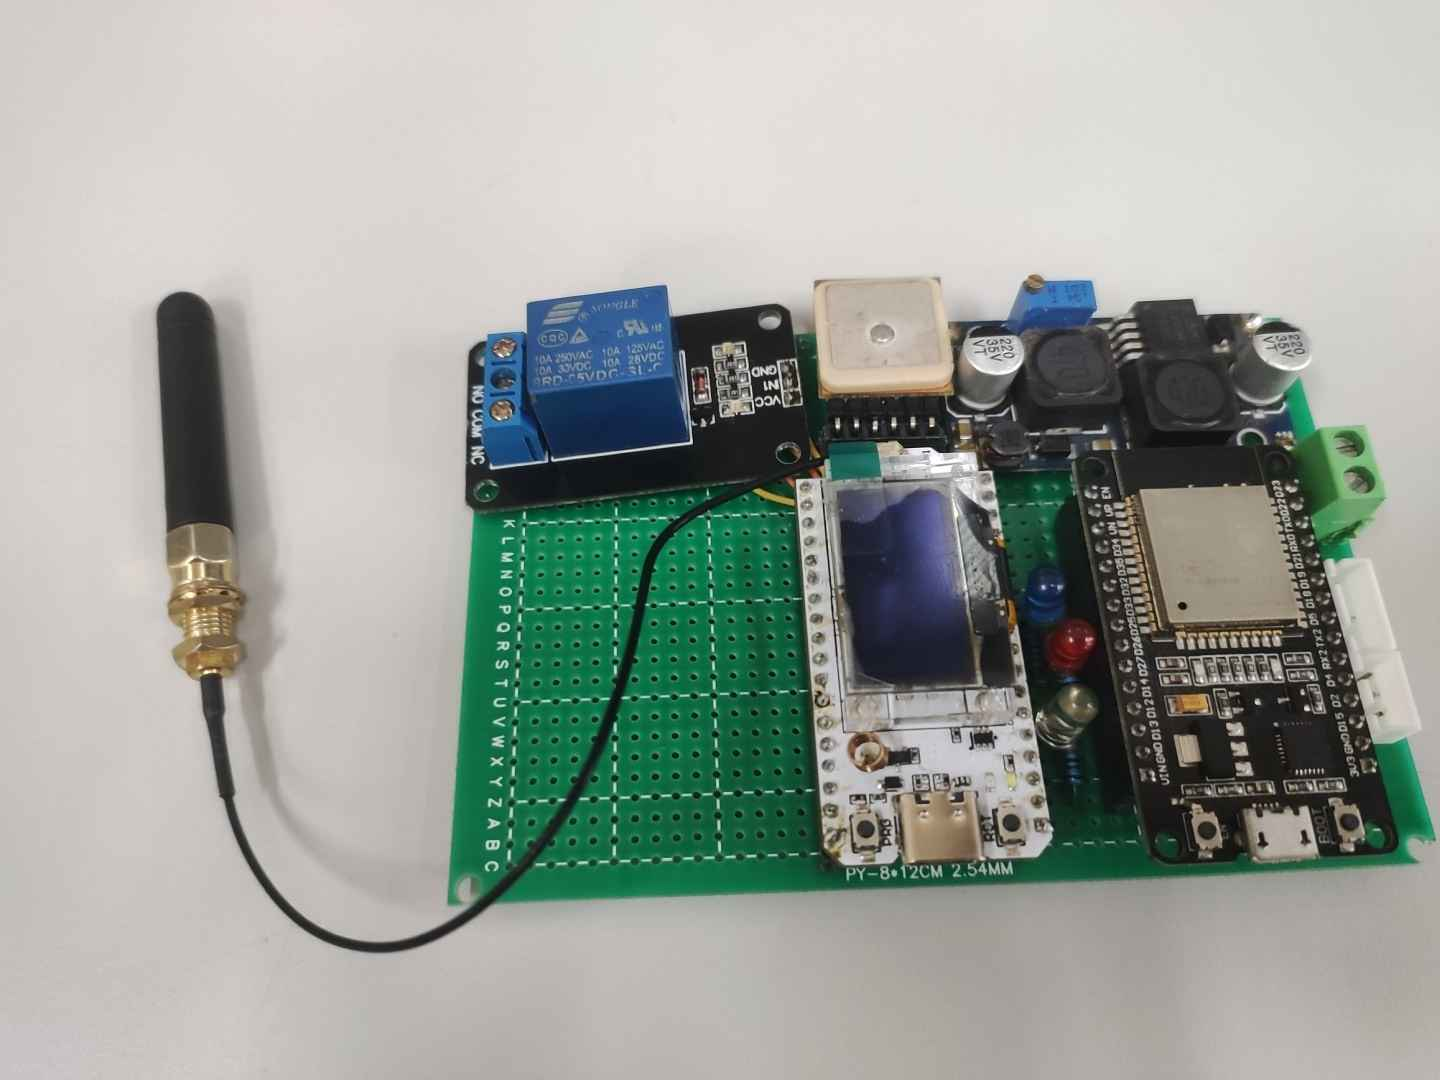
\includegraphics[width=0.7\textwidth]{./capitulo_05/imagen/montajecompleto.jpg}
\caption{Disposición estructural.\label{fig:disposicion}}
\end{center}
\end{minipage}
\end{figure}

En la siguiente Figura \ref{fig:integracion}, se presenta el encapsulado en \textit{3D}, elaborado mediante impresión en una impresora \textit{3D}, el cual proporciona protección y organización a los componentes del sistema. En la Figura \ref{fig:caserfid}, se muestra un encapsulado adicional para el módulo \textit{RFID}.

\begin{figure}[H]
\leavevmode
\begin{minipage}{\textwidth}
\begin{center}
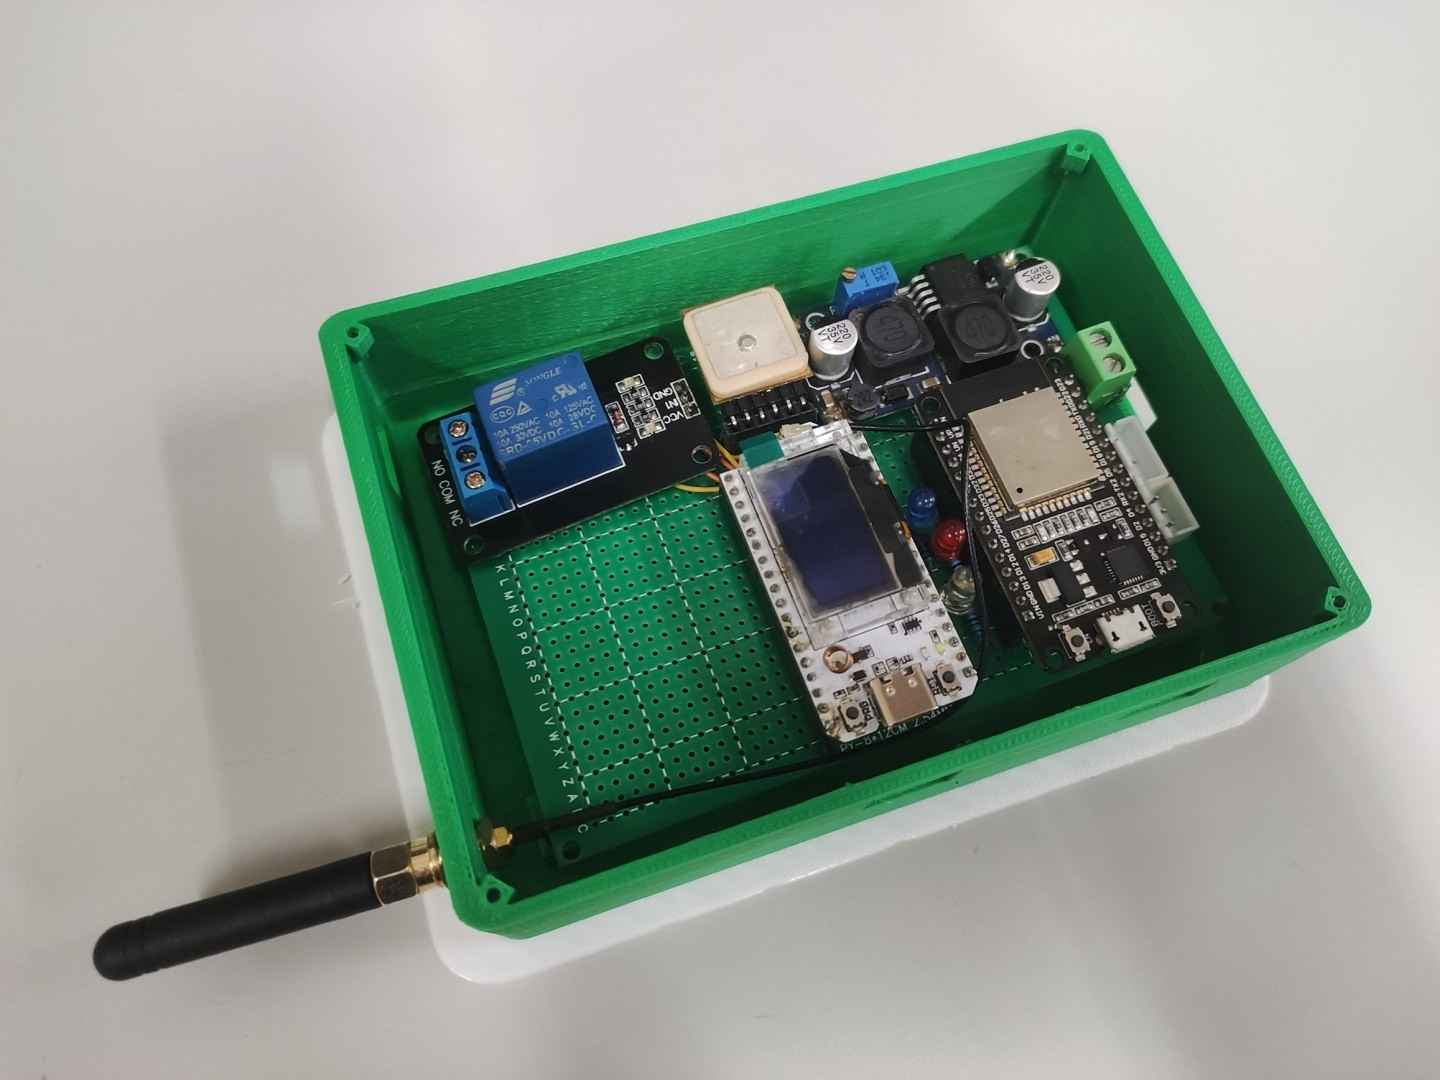
\includegraphics[width=0.7\textwidth]{./capitulo_05/imagen/montajecompleto1.jpg}
\caption{Encapsulado 3D.\label{fig:integracion}}
\end{center}
\end{minipage}
\end{figure}

\begin{figure}[H]
\leavevmode
\begin{minipage}{\textwidth}
\begin{center}
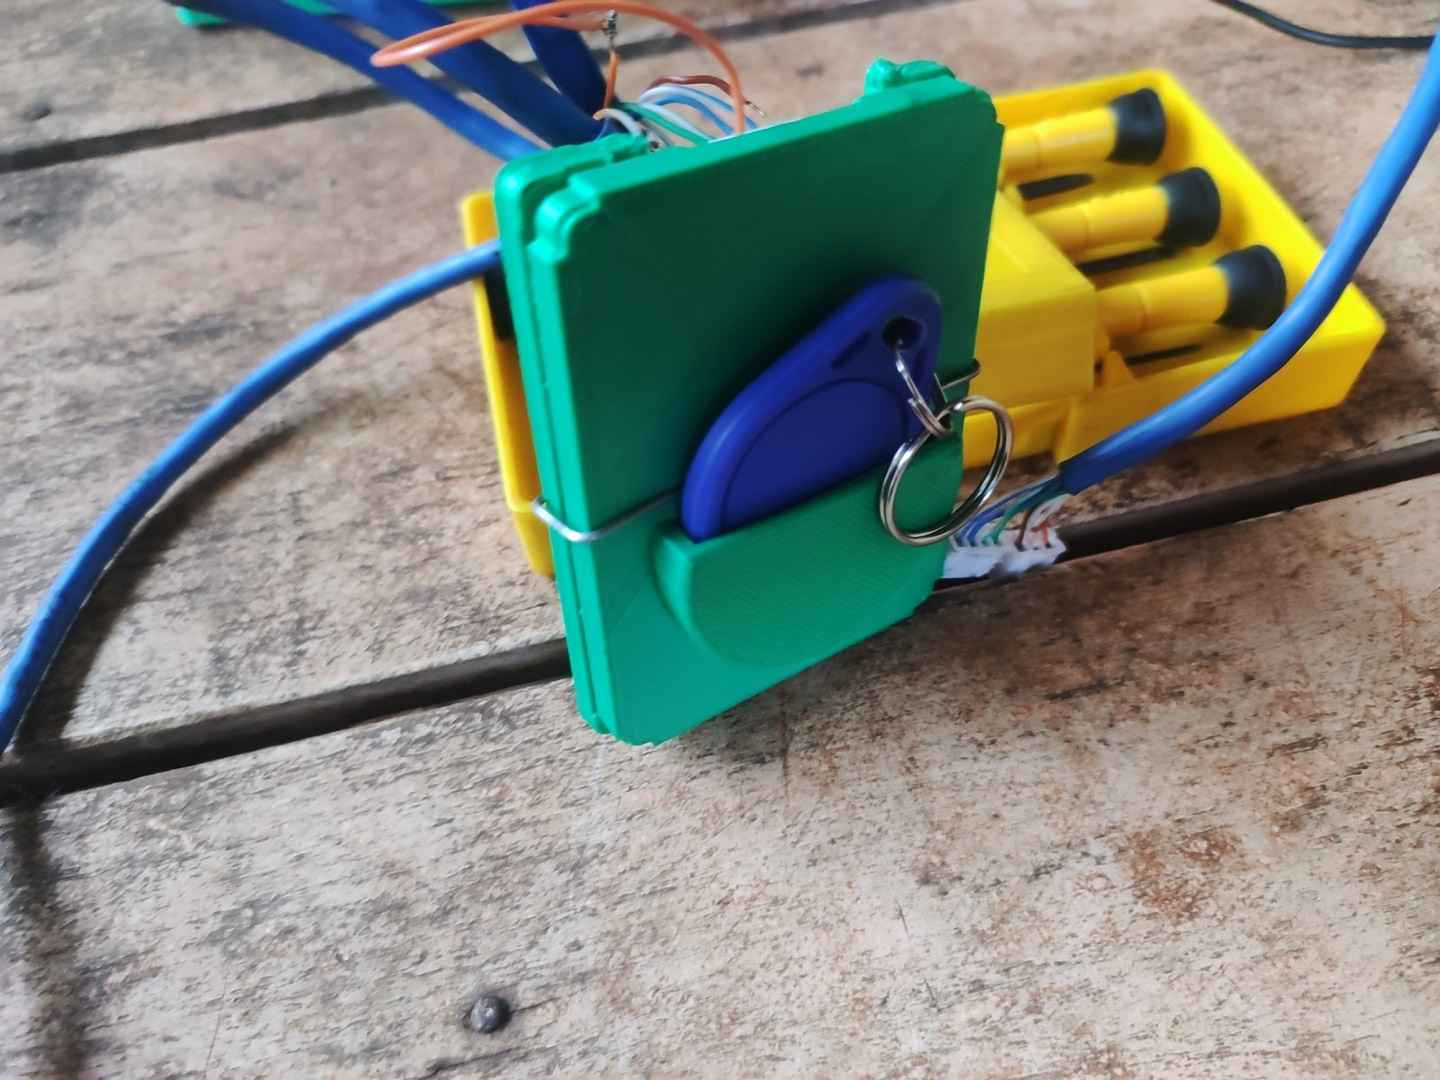
\includegraphics[width=0.6\textwidth]{./capitulo_05/imagen/caserfid.jpg}
\caption{Encapsulado 3D para el módulo \textit{RFID}.\label{fig:caserfid}}
\end{center}
\end{minipage}
\end{figure}

Por último, en la Figura \ref{fig:motocompleto}, se presenta el montaje final del sistema, con todos los componentes integrados y dispuestos en la motocicleta. La Figura \ref{fig:motocompleto} incluye flechas que destacan la ubicación precisa de los prototipos, facilitando su identificación y visualización en el contexto del montaje completo.

\begin{figure}[H]
\leavevmode
\begin{minipage}{\textwidth}
\begin{center}
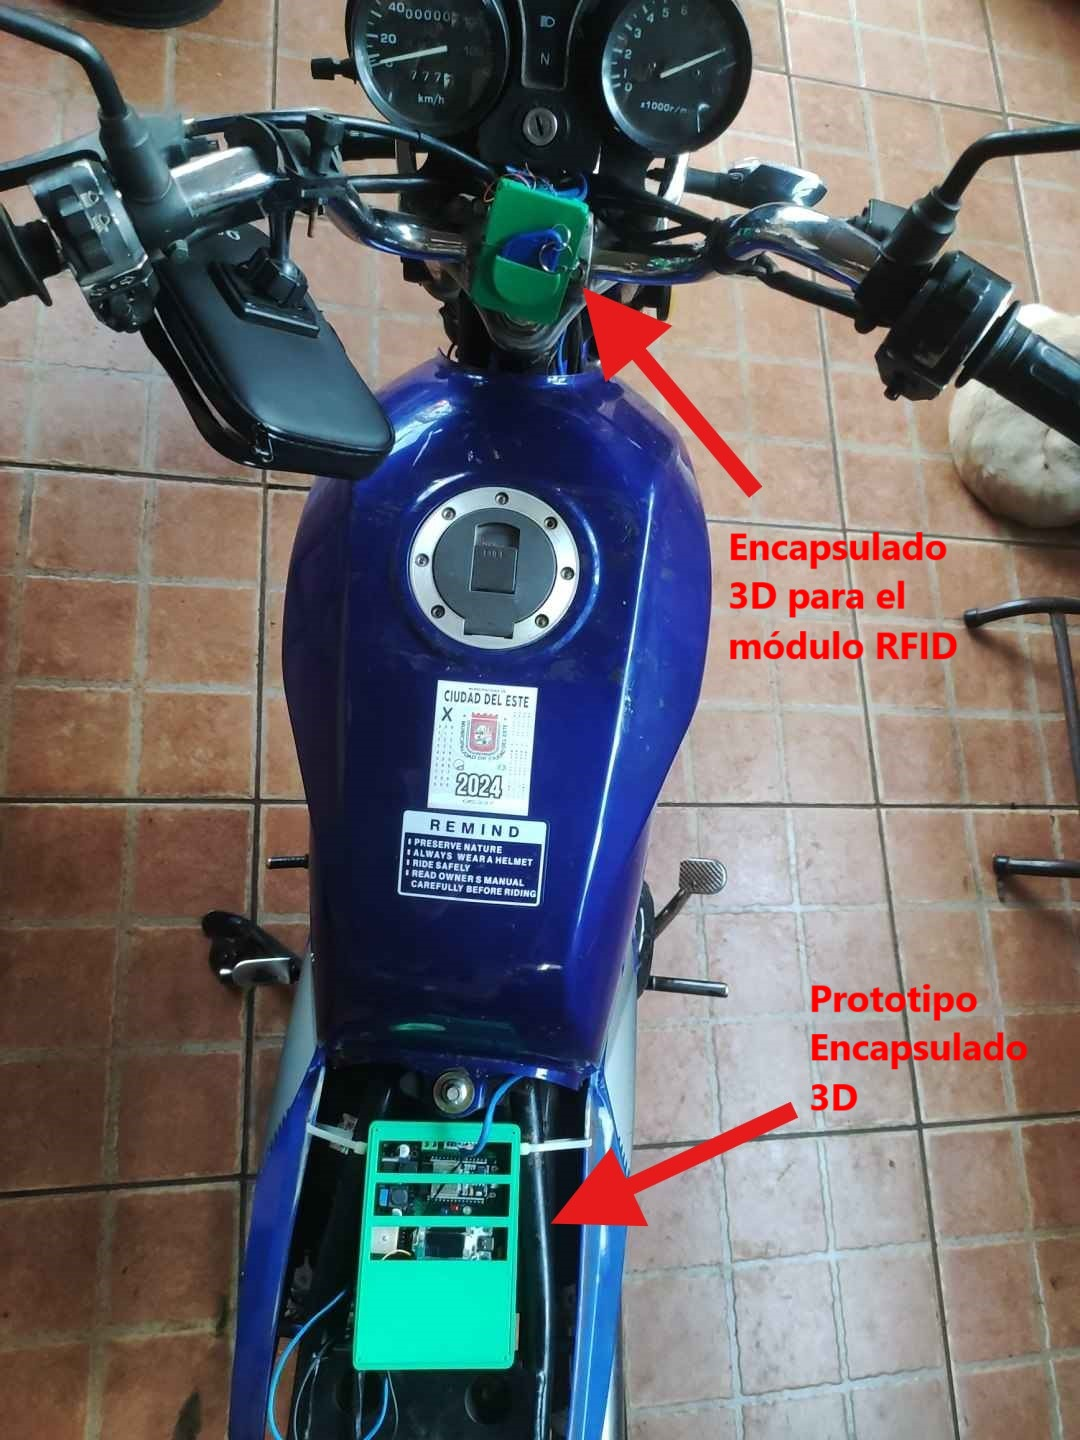
\includegraphics[width=0.5\textwidth]{./capitulo_05/imagen/prototipofinalmontado.jpg}
\caption{Prototipo Final.\label{fig:motocompleto}}
\end{center}
\end{minipage}
\end{figure}

\subsubsection{\textit{Software} del prototipo}

El \textit{software} desarrollado para el prototipo habilita las funciones principales del sistema, asegurando la integración de los módulos de \textit{hardware} con un control eficiente y coordinado. Este \textit{software} gestiona la interacción entre los componentes, facilitando la autenticación de usuarios, el monitoreo continuo y la transmisión de datos mediante \textit{LoRaWAN}.

Entre sus funcionalidades más relevantes, se encuentra la validación de usuarios mediante el lector \textit{RFID}, supervisando de forma constante la presencia del \textit{UID} autorizado. En caso de desconexión, el \textit{software} ejecuta automáticamente acciones críticas, como el corte de energía de la motocicleta, reforzando la seguridad del sistema.\\

Adicionalmente, el \textit{software} es responsable de la recopilación y transmisión de datos relevantes, como las coordenadas \textit{GPS} y el \textit{UID} autenticado, a través de \textit{LoRaWAN}. Esto asegura que el usuario pueda recibir alertas en tiempo real, incluyendo notificaciones de eventos críticos como intentos de arranque no autorizados.

Una de las características más destacadas es la capacidad del \textit{software} para integrar y mostrar estos datos en una plataforma gráfica basada en \textit{ThingsBoard}. En esta interfaz, el usuario puede visualizar la ubicación en tiempo real de la motocicleta sobre un mapa interactivo, además de consultar una tabla de series temporales que detalla las coordenadas transmitidas y otros parámetros relevantes.\\

En la Figura \ref{fig:finresul} se presenta un ejemplo de la visualización en la plataforma, destacando cómo el \textit{software} permite un monitoreo continuo y detallado. La figura muestra la ubicación de la motocicleta y los datos transmitidos mediante \textit{LoRaWAN}.

\begin{figure}[H]
\leavevmode
\begin{minipage}{\textwidth}
\begin{center}
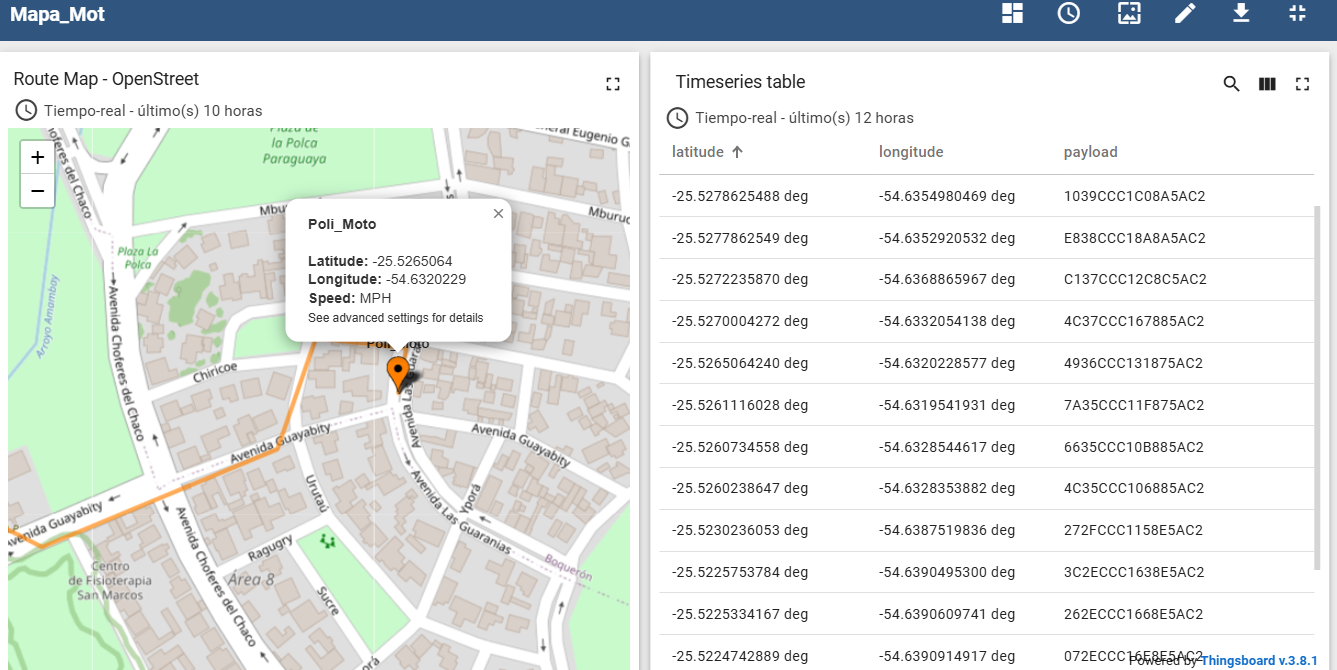
\includegraphics[width=1.0\textwidth]{./capitulo_05/imagen/resulfin.png}
\caption{Visualización de datos en tiempo real.\label{fig:finresul}}
\end{center}
\end{minipage}
\end{figure}

Con estas funcionalidades, el \textit{software} habilita una solución tecnológica que combina seguridad, monitoreo y gestión de datos en tiempo real, respondiendo a las necesidades específicas del prototipo desarrollado.



